\documentclass[a4paper]{report}
% Some basic packages
\usepackage[utf8]{inputenc}
\usepackage[T1]{fontenc}
\usepackage{textcomp}
\usepackage[english]{babel}
\usepackage{url}
\usepackage{graphicx}
\usepackage{float}
\usepackage{booktabs}
\usepackage{enumitem}

\pdfminorversion=7

% Don't indent paragraphs, leave some space between them
\usepackage{parskip}

% Hide page number when page is empty
\usepackage{emptypage}
\usepackage{subcaption}
\usepackage{multicol}
\usepackage{xcolor}

% Other font I sometimes use.
% \usepackage{cmbright}

% Math stuff
\usepackage{amsmath, amsfonts, mathtools, amsthm, amssymb}
% Fancy script capitals
\usepackage{mathrsfs}
\usepackage{cancel}
% Bold math
\usepackage{bm}
% Some shortcuts
\newcommand\N{\ensuremath{\mathbb{N}}}
\newcommand\R{\ensuremath{\mathbb{R}}}
\newcommand\Z{\ensuremath{\mathbb{Z}}}
\renewcommand\O{\ensuremath{\emptyset}}
\newcommand\Q{\ensuremath{\mathbb{Q}}}
\newcommand\C{\ensuremath{\mathbb{C}}}
\renewcommand\L{\ensuremath{\mathcal{L}}}

% Package for Petri Net drawing
\usepackage[version=0.96]{pgf}
\usepackage{tikz}
\usetikzlibrary{arrows,shapes,automata,petri}
\usepackage{tikzit}
\input{petri_nets_style.tikzstyles}

% Easily typeset systems of equations (French package)
\usepackage{systeme}

% Put x \to \infty below \lim
\let\svlim\lim\def\lim{\svlim\limits}

%Make implies and impliedby shorter
\let\implies\Rightarrow
\let\impliedby\Leftarrow
\let\iff\Leftrightarrow
\let\epsilon\varepsilon

% Add \contra symbol to denote contradiction
\usepackage{stmaryrd} % for \lightning
\newcommand\contra{\scalebox{1.5}{$\lightning$}}

% \let\phi\varphi

% Command for short corrections
% Usage: 1+1=\correct{3}{2}

\definecolor{correct}{HTML}{009900}
\newcommand\correct[2]{\ensuremath{\:}{\color{red}{#1}}\ensuremath{\to }{\color{correct}{#2}}\ensuremath{\:}}
\newcommand\green[1]{{\color{correct}{#1}}}

% horizontal rule
\newcommand\hr{
    \noindent\rule[0.5ex]{\linewidth}{0.5pt}
}

% hide parts
\newcommand\hide[1]{}

% si unitx
\usepackage{siunitx}
\sisetup{locale = FR}

% Environments
\makeatother
% For box around Definition, Theorem, \ldots
\usepackage{mdframed}
\mdfsetup{skipabove=1em,skipbelow=0em}
\theoremstyle{definition}
\newmdtheoremenv[nobreak=true]{definitie}{Definitie}
\newmdtheoremenv[nobreak=true]{eigenschap}{Eigenschap}
\newmdtheoremenv[nobreak=true]{gevolg}{Gevolg}
\newmdtheoremenv[nobreak=true]{lemma}{Lemma}
\newmdtheoremenv[nobreak=true]{propositie}{Propositie}
\newmdtheoremenv[nobreak=true]{stelling}{Stelling}
\newmdtheoremenv[nobreak=true]{wet}{Wet}
\newmdtheoremenv[nobreak=true]{postulaat}{Postulaat}
\newmdtheoremenv{conclusie}{Conclusie}
\newmdtheoremenv{toemaatje}{Toemaatje}
\newmdtheoremenv{vermoeden}{Vermoeden}
\newtheorem*{herhaling}{Herhaling}
\newtheorem*{intermezzo}{Intermezzo}
\newtheorem*{notatie}{Notatie}
\newtheorem*{observatie}{Observatie}
\newtheorem*{exe}{Exercise}
\newtheorem*{opmerking}{Opmerking}
\newtheorem*{praktisch}{Praktisch}
\newtheorem*{probleem}{Probleem}
\newtheorem*{terminologie}{Terminologie}
\newtheorem*{toepassing}{Toepassing}
\newtheorem*{uovt}{UOVT}
\newtheorem*{vb}{Voorbeeld}
\newtheorem*{vraag}{Vraag}

\newmdtheoremenv[nobreak=true]{definition}{Definition}
\newtheorem*{eg}{Example}
\newtheorem*{notation}{Notation}
\newtheorem*{previouslyseen}{As previously seen}
\newtheorem*{remark}{Remark}
\newtheorem*{note}{Note}
\newtheorem*{problem}{Problem}
\newtheorem*{observe}{Observe}
\newtheorem*{property}{Property}
\newtheorem*{intuition}{Intuition}
\newmdtheoremenv[nobreak=true]{prop}{Proposition}
\newmdtheoremenv[nobreak=true]{theorem}{Theorem}
\newmdtheoremenv[nobreak=true]{corollary}{Corollary}

% End example and intermezzo environments with a small diamond (just like proof
% environments end with a small square)
\usepackage{etoolbox}
\AtEndEnvironment{vb}{\null\hfill$\diamond$}%
\AtEndEnvironment{intermezzo}{\null\hfill$\diamond$}%
% \AtEndEnvironment{opmerking}{\null\hfill$\diamond$}%

% Fix some spacing
% http://tex.stackexchange.com/questions/22119/how-can-i-change-the-spacing-before-theorems-with-amsthm
\makeatletter
\def\thm@space@setup{%
  \thm@preskip=\parskip \thm@postskip=0pt
}


% Exercise 
% Usage:
% \exercise{5}
% \subexercise{1}
% \subexercise{2}
% \subexercise{3}
% gives
% Exercise 5
%   Exercise 5.1
%   Exercise 5.2
%   Exercise 5.3
\newcommand{\exercise}[1]{%
    \def\@exercise{#1}%
    \subsection*{Exercise #1}
}

\newcommand{\subexercise}[1]{%
    \subsubsection*{Exercise \@exercise.#1}
}


% \lecture starts a new lecture (les in dutch)
%
% Usage:
% \lecture{1}{di 12 feb 2019 16:00}{Inleiding}
%
% This adds a section heading with the number / title of the lecture and a
% margin paragraph with the date.

% I use \dateparts here to hide the year (2019). This way, I can easily parse
% the date of each lecture unambiguously while still having a human-friendly
% short format printed to the pdf.

\usepackage{xifthen}
\def\testdateparts#1{\dateparts#1\relax}
\def\dateparts#1 #2 #3 #4 #5\relax{
    \marginpar{\small\textsf{\mbox{#1 #2 #3 #5}}}
}

\def\@lecture{}%
\newcommand{\lecture}[3]{
    \ifthenelse{\isempty{#3}}{%
        \def\@lecture{Lecture #1}%
    }{%
        \def\@lecture{Lecture #1: #3}%
    }%
    \subsection*{\@lecture}
    \marginpar{\small\textsf{\mbox{#2}}}
}



% These are the fancy headers
\usepackage{fancyhdr}
\pagestyle{fancy}

% LE: left even
% RO: right odd
% CE, CO: center even, center odd
% My name for when I print my lecture notes to use for an open book exam.
% \fancyhead[LE,RO]{Gilles Castel}

\fancyhead[RO,LE]{\@lecture} % Right odd,  Left even
\fancyhead[RE,LO]{}          % Right even, Left odd

\fancyfoot[RO,LE]{\thepage}  % Right odd,  Left even
\fancyfoot[RE,LO]{}          % Right even, Left odd
\fancyfoot[C]{\leftmark}     % Center

\makeatother




% Todonotes and inline notes in fancy boxes
\usepackage{todonotes}
\usepackage{tcolorbox}

% Make boxes breakable
\tcbuselibrary{breakable}

% Verbetering is correction in Dutch
% Usage: 
% \begin{verbetering}
%     Lorem ipsum dolor sit amet, consetetur sadipscing elitr, sed diam nonumy eirmod
%     tempor invidunt ut labore et dolore magna aliquyam erat, sed diam voluptua. At
%     vero eos et accusam et justo duo dolores et ea rebum. Stet clita kasd gubergren,
%     no sea takimata sanctus est Lorem ipsum dolor sit amet.
% \end{verbetering}
\newenvironment{verbetering}{\begin{tcolorbox}[
    arc=0mm,
    colback=white,
    colframe=green!60!black,
    title=Opmerking,
    fonttitle=\sffamily,
    breakable
]}{\end{tcolorbox}}

% Noot is note in Dutch. Same as 'verbetering' but color of box is different
\newenvironment{noot}[1]{\begin{tcolorbox}[
    arc=0mm,
    colback=white,
    colframe=white!60!black,
    title=#1,
    fonttitle=\sffamily,
    breakable
]}{\end{tcolorbox}}




% Figure support as explained in my blog post.
\usepackage{import}
\usepackage{xifthen}
\usepackage{pdfpages}
\usepackage{transparent}
\newcommand{\incfig}[1]{%
    \def\svgwidth{\columnwidth}
    \import{./figures/}{#1.pdf_tex}
}

% Fix some stuff
% %http://tex.stackexchange.com/questions/76273/multiple-pdfs-with-page-group-included-in-a-single-page-warning
\pdfsuppresswarningpagegroup=1


% My name
\author{Bruno M. Pacheco}


\title{EMC5467 - Acionamentos Hidráulicos e Pneumáticos para Automação - P1}

\begin{document}

\textbf{Objetivo do Curso:}
Circuitos de atuação destinados ao controle de posição utilizando válvulas proporcionais ou servoválvulas e cilindros hidráulicos.

\section*{Princípios Físicos Fundamentais}

Um fluido (newtoniano) se caracteriza por respeitar a equação \[
\tau = \mu \frac{\partial v}{\partial y} 
\], em que $\tau$ é a tensão de cisalhamento, $\mu$ é a viscosidade do fluido, $v$ é a velocidade do fluido em relação ao eixo $y$.

Quando o fluido não apresenta variação significativa da sua massa específica para uma dada aplicação, ele é considerado \emph{incompressível}. Do contrário, é considerado \emph{compressível}.

\begin{description}
    \item[Pneumática] utilizam ar comprimido, tratado como \emph{não-viscoso}, e \emph{compressível}.
    \item[Hidráulica] utilizam líquidos, tratados como \emph{viscosos}, e \emph{geralmente incompressíveis}.
\end{description}

\subsection*{Princípio de Pascal}

\emph{"Se uma força externa for aplicada sobre uma parcela de área de um fluido confinado, a pressão decorrente será transmitida integralmente a todo o fluido e à área do recipiente que o contém"}. Em outras palavras, \[
p = \frac{F_1}{A_1} = \frac{F_2}{A_2}
\].

\section*{Sistemas de Autuação Hidráulicos Com Controle Contínuo}

A função dos sistemas de atuação contínua pode ser definida pelo tipo de válvula utilizada, categorizadas em:
\begin{itemize}
    \item Válvulas de controle contínuo de pressão (VCCP)
    \item Válvulas de controle contínuo de vazão (VCCV)
    \item Válvulas de controle contínuo direcional (VCCD)
\end{itemize}

\subsection*{Servoválvulas}

Utilizam motores elétricos para realizar o acionamento, em um ou dois estágios.

\subsection*{Válvulas Direcionais Proporcionais (VDP)}

Utilizam solenóides para realizar o acionamento. Como os solenóides se movimentam em somente um sentido, são necessário utilizar dois solenoides, um em cada extremidade do carretel.

Para aplicações de grande porte (em relação à vazão), utilizam-se válvulas de dois estágios, \emph{i.e.}, a válvula piloto controla o pistão conectado ao carretel da válvula principal, de maior porte.


\section*{Modelagem e Dimensionamento Dinâmico dos Sistemas de Atuação (para circuitos de atuação contínua)}

\subsection*{Válvulas carretel de 4 vias}

Possui duas formas construtivas, diferenciadas pelo número de ressaltos:
\begin{figure}[H]
    \centering
    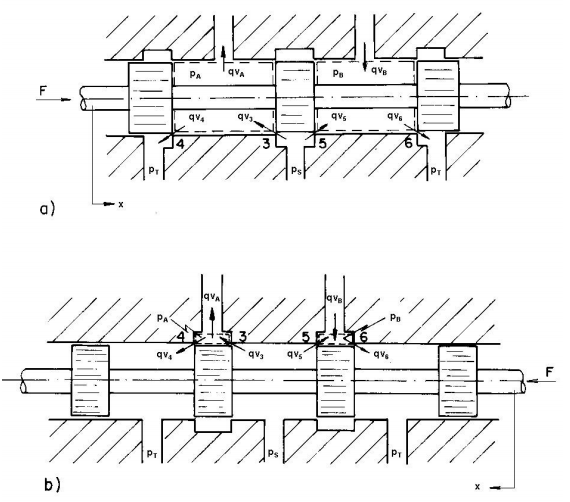
\includegraphics[width=0.6\textwidth]{valvula_carretel_4.png}
\end{figure}
Note que a orientação delas está espelhada.

Pode-se diferenciar as válvulas de acordo com a relação do tamanho do pórtico (abetura para os canais) em relação ao ressalto ("êmbolo"):
\begin{description}
    \item[supercrítico] ressalto maior do que o pórtico $\implies$ existe uma região em que não há passagem de fluido para nenhum canal
    \item[crítico] ressalto exatamente do tamanho do pórtico $\implies$ somente um ponto (hipotético) em que não há passagem de fluido
    \item[subcrítico] ressalto menor do que o pórtico $\implies$ sempre há passagem de fluido para algum canal, existe uma região em que os canais possuem conexão
\end{description}

\subsubsection*{Vazão de controle}

A vazão controlada depende dos 4 orifícios existentes, que agem como constrições para o fluxo. Assim, partimos da equação que estabelece a relação entre a vazão e a queda de pressão em um orifício \[
q_v = C_d A_0 \sqrt{\frac{2\Delta p}{\rho}} 
\], onde $C_d$ é o coeficiente relativo ao orifício, $A_0$ é a área do orifício e $\rho$ é a massa específica do fluido.

Assim, a fórmula para a vazão de controle em uma válvula de 4 vias é \[
q_v = q_{v_A} = q_{v_B} = C_d w x \sqrt{\frac{\Delta p_t}{\rho}} 
\], onde $\Delta p_t = p_S - p_T - sgn\left( x \right) p_C$ ou $\Delta p_t = p_S - \left( p_A - p_B \right)$, $w$ é a largura do orifício, e $p_c$ é a pressão de carga, definida como $p_C = p_A - p_B$.

Uma informação típica fornecida é a vazão nominal da válvula, normalmente na forma de curvas. Essas curvas caracterizam a equação \[
q_{v_n} = C_d w x_n \sqrt{\frac{p_S}{\rho}} 
\], resultante de ensaios com $p_C = 0$. Assim, podemos encontrar a fórmula \[
q_v = K_v \frac{x}{x_n}\sqrt{\Delta p_t} 
\], onde \[
K_v = \frac{q_{v_n}}{\sqrt{\Delta p_{t_n}} }
\] 

Podemos linearizar essa equação em torno de um ponto de operação, obtendo a equação \[
q_v = K_{q_0}x - K_{C_0}p_C
\], onde \[
K_{q_0} = \frac{\partial q_v}{\partial x} \bigg\rvert_0 = C_d w \sqrt{\frac{p_S}{\rho}} 
\] é o ganho de vazão e \[
K_{C_0} = \frac{\partial q_v}{\partial p_C} \bigg\rvert_0 = \frac{\pi w f_r^2}{32\mu}
\] é o ganho de pressão, onde $f_r$ a folga radial e $\mu$ a viscosidade absoluta do fluido. Também pode-se obter os ganhos a partir das curvas vazão-pressão do fornecedor.

Uma forma mais segura, entretanto, de se obter esses coeficientes é através de ensaios. Para determinar o ganho de vazão, conecta-se um transdutor de vazão entre as portas A-B. Para determinar o ganho de pressão, conectam-se dois transdutores de pressão nas mesmas portas.

\subsubsection*{Movimento do Carretel}

Apesar da diferença construtiva entre o solenóide proporcional e o motor de torque, é possível obter um modelo dinâmico único adequado para a análise de sistemas de controle. Podemos modelar a relação entre a tensão de controle e a corrente como \[
U_c(t) = L \frac{di}{dt}(t) + R i(t)
\], assim modelando a relação entre o sinal de entrada e a corrente gerada, que é fundamental para modelar a ação desses componente. Para o motor de torque, a relação entre o torque $T$ gerado e o deslocamento angular $\theta$ pode ser modelado por \[
T(t) = K_t i(t) = I \frac{d^2\theta}{dt^2}(t) + A \frac{d\theta}{dt}(t) +G\theta
\], enquanto no solenóide nos interessa entender a relação entre a força $F$ gerada e o deslocamento linear $x$, \[
F(t) = K_f i(t) = M \frac{d^2x}{dt^2}(t) + B \frac{dx}{dt}(t) +K_x x
\], onde $F(t)$ é a força necessária para movimentar o carretel, $M$ é a massa do carretel, $B$ é o coeficiente de atrito viscoso, $K_x$ é a rigidez, e $F_a$ é a força de atrito.

Podemos, então, definir a resposta dinâmica do carretel com operadores diferenciais \[
K_f U_c(t) = \left( M \mathcal{D}^2 + B \mathcal{D} + K_x \right) \cdot \left( L\mathcal{D} + R \right) x(t)
\]. Caracterizando esse sistema com parâmetros de 2ª ordem, obtemos o modelo \[
K_{RP}U_c(t) = \frac{1}{\omega_n^2}\frac{d^2x}{dt^2}(t) + \frac{2\zeta}{\omega_n}\frac{dx}{dt}(t) + x(t)
\]. Com parâmetros de 1ª ordem, obtemos o modelo \[
K_{RP}U_c(t) = \tau \frac{dx}{dt}(t) + x(t)
\].

\begin{figure}[H]
    \centering
    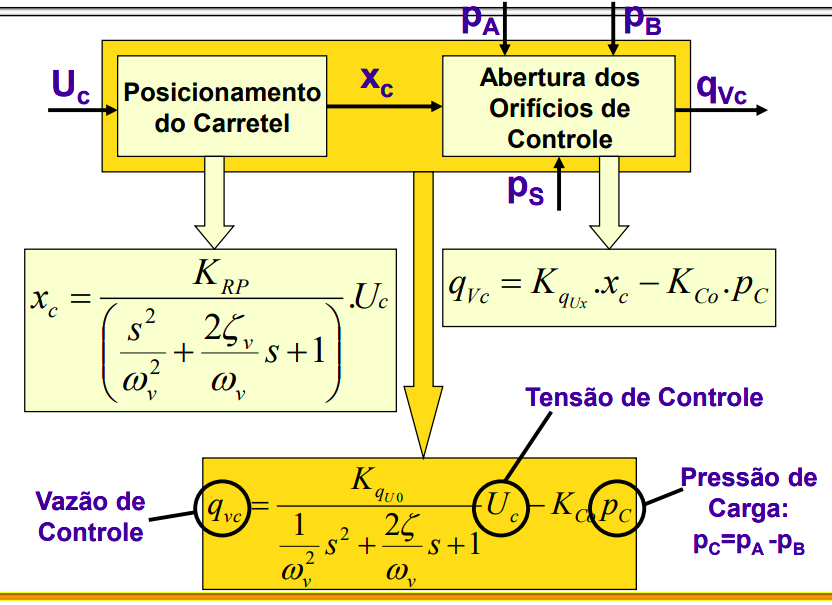
\includegraphics[width=0.6\textwidth]{esquema_valvula_carretel.png}
\end{figure}

\subsection*{Cilindros de dupla ação simétricos}

Duas equação são fundamentais para entendermos o comportamento de um cilindro de dupla ação simétrico.

\begin{figure}[H]
    \centering
    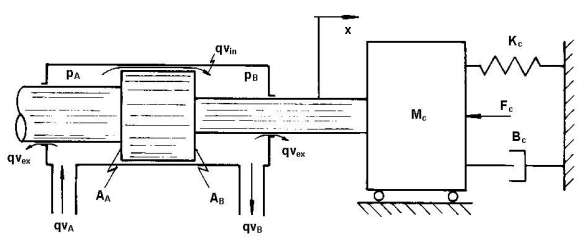
\includegraphics[width=0.8\textwidth]{cilindro_dupla_acao.png}
\end{figure}

\subsubsection*{Equação da Continuidade}

\begin{figure}[H]
    \centering
    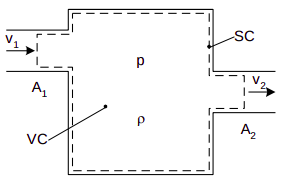
\includegraphics[width=0.5\textwidth]{equacao_continuidade.png}
\end{figure}

Temos que a diferença entre as vazões em um volume de controle VC conforme a imagem acima segue \[
q_{v_1} - q_{v_2} = \frac{dV}{dt}(t) + \frac{V}{\beta}(t) \frac{dp}{dt}(t)
\], onde $\beta$ é o coeficiente de compressibilidade do fluido.

Aplicando essa equação ao cilindro, temos \[
q_{VC} = C_{in}p_C + A \frac{dx}{dt} + \frac{V_t}{4\beta}\frac{dp_C}{dt}
\], onde $C_{in}$ é o coeficiente de vazão interna $q_{V_{in}}$, $p_C = p_A - p_B$ e $V_t = V_A + V_B$ é o volume total.

\subsubsection*{Equação do Movimento}

Podemos modelar o movimento do êmbolo do cilindro através da força necessária \[
F = Ap_C = M_C \frac{d^2x}{dt} + B_C \frac{dx}{dt} + K_C x + F_C
\]. Lembrando que é necessária uma diferença de pressão para vencer a inércia do sistema.

\subsubsection*{Modelo}

A partir dessas duas equações é possível modelar a posição do cilindro como um sistema de segunda ordem tradicional. Considerando entrada nula (em um ponto de operação), temos que o sistema age de acordo com o modelo \[
    \frac{M_t}{\beta \left( \frac{A_A^2}{V_A} + \frac{A_B^2}{V_B} \right) } \frac{d^2x}{dt^2} + x = 0
\], ou seja, a frequência natural do sistema é \[
\omega_n = \sqrt{\frac{\beta}{M_t} \left( \frac{A_A^2}{V_A} + \frac{A_B^2}{V_B} \right)} 
\], de onde extraímos o coeficiente de rigidez hidráulico de um cilindro \[
K_H = \beta \left( \frac{A_A^2}{V_A} + \frac{A_B^2}{V_B} \right)
\], refraseando, então, $\omega_n = \sqrt{\frac{K_H}{M_t}}$.

Utilizamos a frequência natural do sistema para entender a velocidade do sistema, \emph{i.e.}, quanto maior a frequência natural, maior a velocidade de resposta.

\subsection*{Motores Hidráulicos}

Utilizados como fonte de energia para o circuito, estabelecem uma relação entre o torque do motor e a pressão de entrada/saída através do deslocamento volumétrico, conforme \[
T = Dp_i
\], onde $T$ é o torque no eixo, $D$ é o deslocamento volumétrico medido em volume por rotação ou por ângulo, e $p_i$ é a pressão na entrada ($p_1$), no caso de um motor, ou saída ($p_2$), no caso de um bomba.

Podemos calcular a vazão $q_v$ de uma bomba ou motor através de \[
q_v = D\omega = D \frac{d\theta}{dt}
\], onde $\omega$ é a velocidade angular relativa ao angulo $\theta$ do eixo.

Como o deslocamento volumétrico assume um papel similar ao da área no caso dos cilindros, a modelagem se torna bastante similar.

\subsubsection*{Equação da Continuidade}

Sendo $A$ a câmara de entrada e $B$ a câmara de saída, podemos modelar a vazão de controle \[
q_{V_C} = \frac{q_{V_A}+q_{V_B}}{2}
\] como \[
q_{V_C} = C_{in}p_{C} + D \frac{d\theta}{dt} + \frac{V_t}{4\beta} \frac{d p_C}{dt}
\], bastante similar ao cilindro.

\subsubsection*{Equação do Movimento}

A partir da equação do torque exercido, podemos modelar o movimento através da relação do torque com a pressão $C$ e o deslocamento volumétrico, ou seja, \[
T = D p_C = I \frac{d^2\theta}{dt^2} + A \frac{d\theta}{dt} +G\theta + T_C
\], onde $T_C$ é o torque da carga.

\section*{Sistemas Hidráulicos de Controle de Posição}

\subsection*{Mecânico-Hidráulico}

\begin{figure}[H]
    \centering
    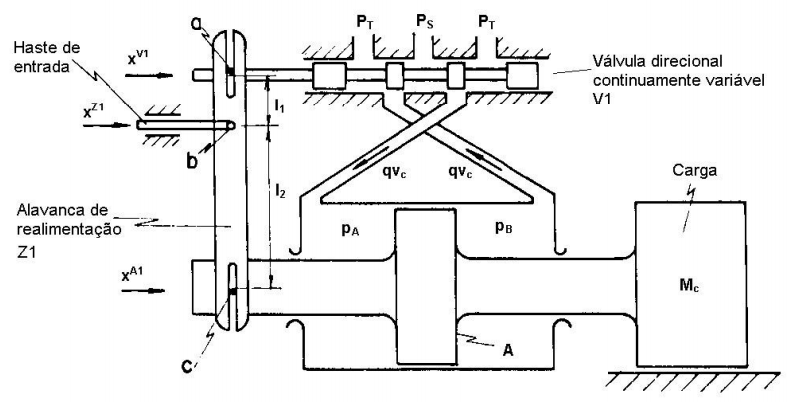
\includegraphics[width=0.8\textwidth]{sistema_mecanico_hidraulico.png}
\end{figure}

Note que $x^{Z_1}$ age como a referência do sistema.

\subsubsection*{Válvula direcional proporcional ou servoválvula (V1)}

Como o "sinal de entrada" para a válvula neste sistema é o deslocamento do carretel, podemos modelar ela somente com a equação da vazão de controle, ou seja, \[
q_{V_C} = K_{q_0}x^{V1} - K_{C_0}p_C
\], onde os ganhos são conhecidos ou obtidos através de ensaios.

\subsubsection*{Cilindro hidráulico e carga (A1)}

Desprezando os vazamentos internos do cilindro, obtemos a equação da continuidade do cilindro \[
q_{V_C} = A \frac{dx^{A1}}{dt} + \frac{V_t}{4\beta} \frac{dp_C}{dt}
\].

Supondo forças de atrito desprezíveis frente a inércia da carga, temos que o movimento do cilindro pode ser descrito pela equação \[
Ap_C = M \frac{d^2x^{A1}}{dt^2}
\].

\subsubsection*{Alavanca de realimentação (Z1)}

Podemos modelar a relação entre os deslocamentos $x^{*}$ considerando constantes as distâncias $I_1$ e $I_2$ pela equação \[
x^{V1} = \frac{I_1 + I_2}{I_2}x^{Z1} - \frac{I_1}{I_2}x^{A1}
\].

\subsubsection*{Modelo do sistema}

\begin{figure}[H]
    \centering
    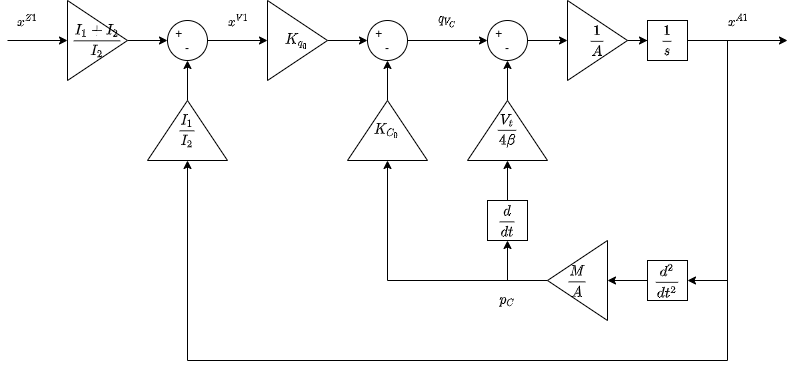
\includegraphics[width=0.8\textwidth]{modelo_mecanico_hidraulico.png}
\end{figure}

Podemos combinar as equações para modelar o conjunto válvula-atuador-carga no domínio da frequência complexa como \[
    \frac{X^{A1}}{X^{V1}}(s) = \frac{K_{RP}}{s\left( \frac{1}{\omega_n^2}s^2 + \frac{2\zeta}{\omega_n}s + 1 \right) }
\], onde
\begin{itemize}
    \item $\omega_n = \sqrt{\frac{4\beta}{V_t}\frac{A^2}{M_c}}$ é a frequência natural do sistema;
	\item $\zeta = \frac{K_{C_0}}{A}\sqrt{\frac{\beta M_c}{V_t}}$ a razão de amortecimento; e
	    \item $K_{RP} = \frac{K_{q_0}}{A}$ é o ganho de regime permanente.
\end{itemize}

Assim, modelamos o sistema final a partir da equação simples da realimentação feita com a haste $Z1$, que só depende da relação entre $I_1$ e $I_2$.

A estabilidade do sistema pode ser garantida se \[
\zeta > \frac{K_{q_0}}{A}\frac{I_1}{I_2}\frac{1}{2\omega_n}
\], ou seja, podemos controlar a estabilidade do sistema através do ganho $\frac{I_1}{I_2}$.

\subsection*{Eletro-Hidráulico}

\begin{figure}[H]
    \centering
    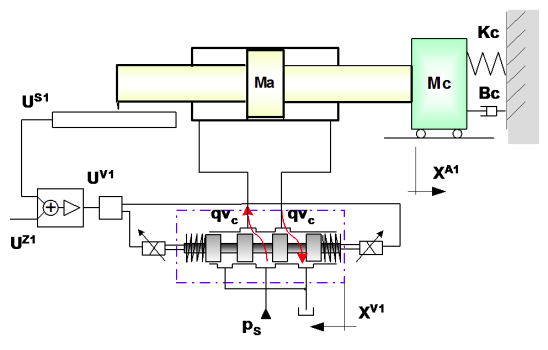
\includegraphics[width=0.8\textwidth]{sistema_eletro_hidraulico.png}
\end{figure}

O objetivo do sistema é controlar a posição $x^{A1}$ através do sinal $U^{Z1}$.

\subsubsection*{Válvula direcional proporcional ou servoválvula (V1)}

Equação da vazão de controle: \[
q_{V_C} = K_{q_0}x^{V_1} - K_{C_0}p_C
\].

Equação do movimento: \[
\left( \frac{1}{\omega_n^2}\mathcal{D}^2 + \frac{2\zeta}{\omega_n}\mathcal{D} + 1 \right) x^{V1} = K^{V 1}U^{V 1}
\].

\subsubsection*{Cilindro hidráulico e carga (A1)}

Novamente, desprezam-se os vazamentos e obtém-se \[
q_{V_C} = A \frac{dx^{A 1}}{dt} + \frac{V_t}{4\beta} \frac{d p_C}{dt}
\].

Considerando o atrito viscoso como significante em relação à inércia da carga, tem-se \[
    Ap_C = M \frac{d^2x^{A 1}}{dt^2} + B \frac{d x^{A 1}}{dt}
\].

\subsubsection*{Sensor de posição (S1)}

O sensor de posição geralmente é um transdutor linear, ou seja, pode ser modelado como \[
U^{S 1} = K^{S 1}x^{A 1}
\] onde $K^{S 1}$ é o ganho do sensor e corresponde à constante de realimentação do sistema.

\subsubsection*{Comparador/Amplificador (Z1)}

O comparador é o elemento que compara os sinais de referência e do sensor e gera o sinal de erro. O amplificador recebe o sinal de erro e amplifica-o para a tensão de trabalho que será aplicada ao mecanismo da válvula. Assim, esses componentes podem ser modelados juntos como \[
U^{V 1} = K^{Z 1}\left( U^{Z 1} - U^{S 1} \right) 
\], onde $K^{Z 1}$ é o ganho de amplificação.

\subsubsection*{Modelo}

\begin{figure}[H]
    \centering
    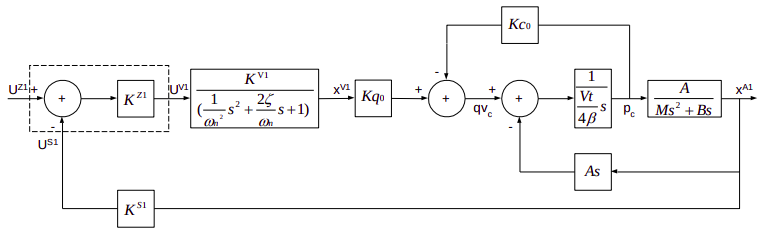
\includegraphics[width=0.8\textwidth]{modelo_eletro_hidraulico.png}
\end{figure}

\section*{Conversão de Unidades}

\begin{table}[H]
    \centering
    \caption{Conversão de unidades}
    \label{tab:label}
    \begin{tabular}{c | c}
      & SI \\
    \hline
    $1$ bar & $1\cdot 10^{5}$ Pa \\
    $1$ St & $1\cdot 10^{-4} \frac{\text{m}^2}{\text{s}}$ \\
    \end{tabular}
\end{table}

\end{document}
